\chapter{LAB 03: Synchronization in OS161}

\section{Introduction to Synchronization}
Modern operating systems are inherently concurrent. Multiple processes or kernel threads often attempt to read and write to the same shared memory structures simultaneously. Without proper orchestration, this concurrency leads to three primary issues:
\begin{itemize}
    \item \textbf{Race Conditions}: The final state of the data depends unpredictably on the exact sequence in which the threads were scheduled.
    \item \textbf{Deadlocks}: Multiple threads block each other indefinitely, each waiting for resources held by another, creating a circular dependency.
    \item \textbf{Resource Starvation}: A thread, although completely valid, is perpetually bypassed by other threads and never gains access to the shared resource.
\end{itemize}

\begin{figure}[h]
    \centering
    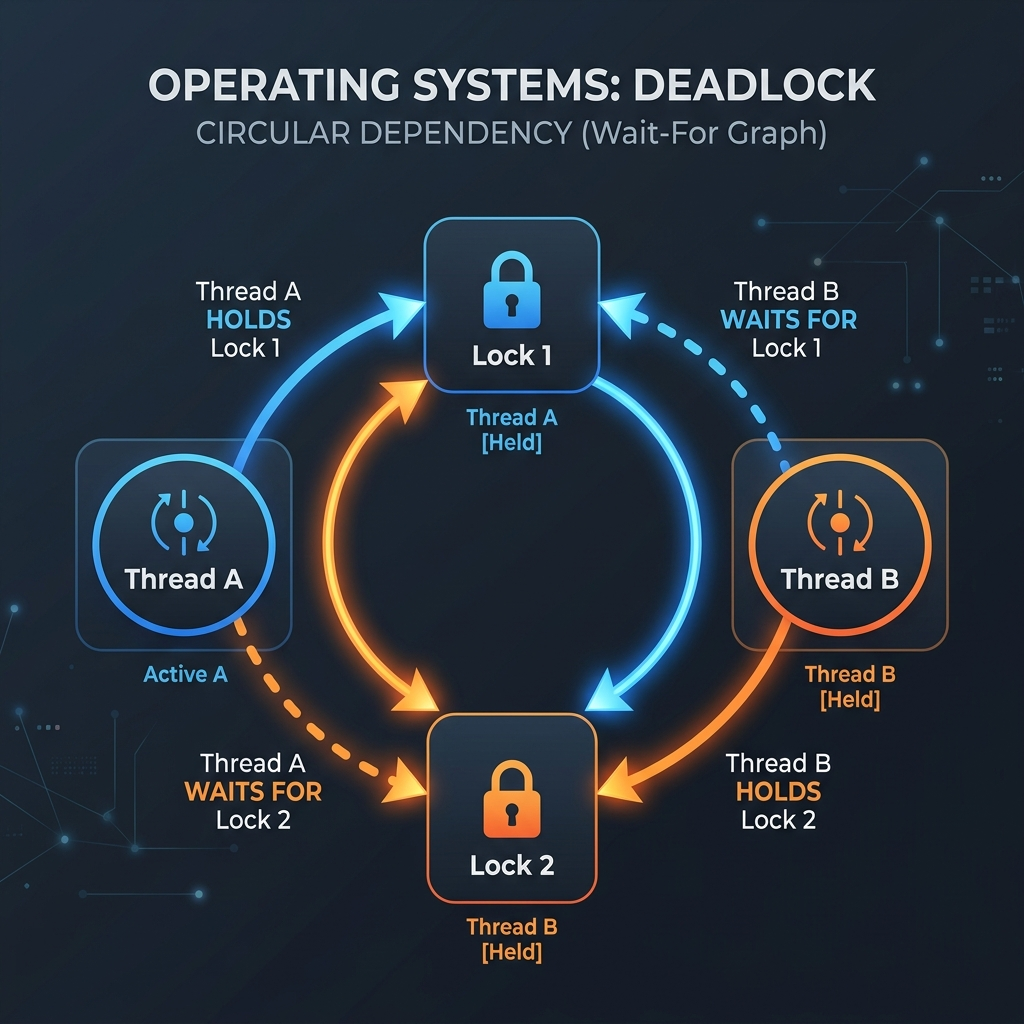
\includegraphics[width=0.7\textwidth]{images/deadlock_diagram.png}
    \caption{A classic Deadlock scenario with circular dependency.}
    \label{fig:deadlock}
\end{figure}

Synchronization primitives are the tools provided by the operating system to prevent these chaotic scenarios. They enforce mutual exclusion (ensuring only one thread accesses a critical section at a time) and coordination (allowing threads to wait for specific events). In OS161, we explore these tools in increasing levels of abstraction: from raw hardware support to Spinlocks, Wait Channels, Semaphores, Locks, and Condition Variables.

\section{Hardware Support: Disabling Interrupts vs. Spinlocks}

\subsection{Software Solutions: Peterson's Algorithm and Limitations}
Before hardware primitives became standard, mutual exclusion could be implemented entirely in software using algorithms like \textbf{Peterson's Solution}. It uses a \texttt{turn} variable and a \texttt{flag} array to coordinate two threads. However, Peterson's algorithm is unreliable on modern architectures due to:
\begin{itemize}
    \item \textbf{Out-of-Order Execution}: Processors reorder instructions to optimize performance, breaking the strict sequencing Peterson's algorithm relies on.
    \item \textbf{Cache Consistency}: Memory writes by one core might not be immediately visible to another.
\end{itemize}
To fix this in weakly-ordered systems, \textbf{Memory Barriers} are used to force the processor to complete all pending memory operations before proceeding. However, for true scalability and ease of use, hardware atomic instructions are preferred.

\subsection{The Limitation of Disabling Interrupts}
A naïve approach to protecting a critical section is simply to disable interrupts (e.g., using \texttt{splhigh()} in OS161) before accessing shared data, and re-enable them (\texttt{splx()}) afterward. If interrupts are disabled, the CPU cannot receive the timer interrupt that triggers a context switch, meaning the current thread cannot be preempted.

While this approach works perfectly on a single-core machine, it completely fails on modern multi-core processors. Disabling interrupts is a \textit{local} operation; it only stops the current CPU from switching threads. It does absolutely nothing to prevent a thread running concurrently on CPU 2 from accessing the same shared memory. Thus, multi-core mutual exclusion requires specialized hardware support in the form of atomic instructions.

\subsection{Spinlocks and the Test-and-Set Instruction}

\begin{tcolorbox}[colback=red!5!white, colframe=red!75!black, title=\textbf{! EXAM FOCUS: IMPLEMENTATION REQUIRED}]
\textbf{Function:} \texttt{spinlock\_acquire(struct spinlock *splk)} \\
\textbf{Exam Task:} \textit{Line-by-Line Analysis \& Bug Detection} \\
Exams ask why \texttt{spinlock\_acquire} utilizes both \texttt{spinlock\_data\_get} and \texttt{spinlock\_data\_testandset} in its inner loop (to reduce atomic bus-locking traffic when the lock is already held). You may also be asked to analyze a flawed \texttt{spinlock\_acquire2} to spot missing optimizations or synchronization bugs.
\end{tcolorbox}

To guarantee mutual exclusion across multiple cores, hardware provides atomic operations like \texttt{test-and-set}. A \textbf{Spinlock} is the lowest-level synchronization primitive built on this hardware support.

A spinlock implements \textit{busy-waiting}. If a thread attempts to acquire a spinlock that is already held, it does not go to sleep; instead, it enters a tight loop (it "spins"), continuously probing the lock's status until it becomes available.

\begin{lstlisting}[language=C]
struct spinlock {
    volatile spinlock_data_t splk_lock; /* The actual hardware lock flag */
    struct cpu *splk_holder;            /* The CPU currently holding the lock */
};
\end{lstlisting}
\textbf{Explanation of the Fields:}
\begin{itemize}
    \item \texttt{splk\_lock}: This is the low-level integer variable that physically represents the lock state (0 for free, non-zero for held). The \texttt{volatile} keyword is essential because it ensures the compiler does not aggressively cache this value in a register, forcing it to read the true value from RAM every time (crucial for polling).
    \item \texttt{splk\_holder}: A pointer to the CPU currently holding the spinlock. It is primarily used for debugging and catching recursive locks (if the same CPU tries to acquire a spinlock it already holds, the kernel panics to prevent an immediate deadlock).
\end{itemize}

In OS161, acquiring a spinlock (\texttt{spinlock\_acquire}) uses two distinct hardware operations in sequence: \texttt{spinlock\_data\_get()} and \texttt{spinlock\_data\_testandset()}. 

\begin{tcolorbox}[colback=blue!5!white,colframe=blue!75!black,title=Exam Insight: Spinlock Implementation (e.g. Q4 2022-09-08)]
Exams often ask you to compare two implementations of \texttt{spinlock\_acquire}:
\begin{itemize}
    \item \textbf{Implementation A (Test-and-Set):} Uses only a \texttt{while} loop executing the expensive \texttt{spinlock\_data\_testandset()} operation continuously. 
    \item \textbf{Implementation B (Test-and-Test-and-Set):} Uses an outer loop with \texttt{spinlock\_data\_testandset()}, and an inner \texttt{while} loop executing the cheaper \texttt{spinlock\_data\_get(\&splk->splk\_lock)}.
\end{itemize}

\textbf{Why is Implementation B (the call to \texttt{spinlock\_data\_get}) strictly necessary?} \\
\texttt{testandset} is an expensive atomic write operation that locks the hardware memory bus. If multiple CPUs constantly execute \texttt{testandset} in a tight loop while waiting for a lock, they will flood the memory bus with write traffic, crippling the performance of the entire system. 

By adding the inner \texttt{spinlock\_data\_get()} loop, the CPU performs a cheap, cacheable read. The CPU spins entirely locally on this read operation using its local cache, without touching the memory bus. Only when the read indicates the lock \textit{might} be free does the CPU break the inner loop and attempt the expensive \texttt{testandset} to actually grab the lock. This drastically reduces bus contention.
\end{tcolorbox}

\subsection{Advanced Hardware Instructions: Compare-and-Swap (CAS)}
While \texttt{test-and-set} is fundamental, modern architectures also provide \textbf{Compare-and-Swap (CAS)}. CAS takes three parameters: a memory location, an expected value, and a new value. It atomically reads the location and, \textit{only if} it matches the expected value, updates it to the new value. 
This is more powerful than \texttt{test-and-set} because it avoids unnecessary memory writes and can handle arbitrary values. CAS is the building block for \textbf{Atomic Variables} (like \texttt{atomic\_int}), allowing counters to be safely incremented without full locks by retrying the CAS in a loop until it succeeds. It can also be used with an array of waiting flags to create advanced fair locks that prevent starvation.

Because spinlocks employ busy-waiting (wasting CPU cycles), they must only be used to protect extremely short critical sections where the wait time is expected to be minimal. 


\section{The Sleeping Engine: Wait Channels (\texttt{wchan})}
For longer waiting periods (e.g., waiting for disk I/O or waiting for a long computation), busy-waiting is unacceptable. The thread must relinquish the CPU and enter the \texttt{SLEEP} state. In OS161, this is achieved using \textbf{Wait Channels}.

A wait channel is essentially a queue of sleeping threads. The fundamental operations are:
\begin{itemize}
    \item \texttt{wchan\_sleep(struct wchan *wc, struct spinlock *lk)}: Puts the current thread to sleep on the wait channel.
    \item \texttt{wchan\_wakeone(struct wchan *wc, struct spinlock *lk)}: Awakens exactly one thread (if any are sleeping).
    \item \texttt{wchan\_wakeall(struct wchan *wc, struct spinlock *lk)}: Awakens all threads sleeping on the channel.
\end{itemize}

\subsection{The Spinlock Sleep Deadlock}
A critical and frequently tested design choice is why \texttt{wchan\_sleep} requires a spinlock as a parameter.
When a thread decides it needs to sleep, it must protect the operation of inserting itself into the wait channel's queue. To ensure mutual exclusion on this queue, the thread must hold a spinlock. 

However, a fundamental rule of kernel programming is: \textbf{You must never go to sleep while holding a spinlock}. If Thread A holds a spinlock and goes to sleep, and Thread B attempts to acquire that same spinlock, Thread B will spin infinitely (busy-waiting) because Thread A can never run to release it. This is a fatal deadlock.

Therefore, the spinlock must be released right as the thread goes to sleep. But if the thread releases the spinlock \textit{before} calling \texttt{wchan\_sleep}, a race condition occurs: another thread could fire a wakeup signal in that tiny window before the thread actually sleeps, causing the signal to be lost forever.

The solution is to pass the held spinlock \textit{into} \texttt{wchan\_sleep}. The \texttt{wchan\_sleep} function performs the context switch and, atomically inside the deep assembly logic of the scheduler, releases the spinlock exactly at the moment the thread transitions into the sleep state. When the thread is later awakened, \texttt{wchan\_sleep} reacquires the spinlock before returning to the caller.

\section{Semaphores vs. Locks}
Moving up in abstraction, OS161 provides Semaphores and Locks. Both implement \textit{non-busy waiting} (they put threads to sleep using wait channels if the resource is unavailable).

\subsection{Semaphores}

\begin{tcolorbox}[colback=red!5!white, colframe=red!75!black, title=\textbf{! EXAM FOCUS: IMPLEMENTATION REQUIRED}]
\textbf{Function:} \texttt{P(struct semaphore *sem) \& V(struct semaphore *sem)} \\
\textbf{Exam Task:} \textit{Line-by-Line Analysis} \\
You must be able to explain the internal implementation of \texttt{P()} and \texttt{V()}: Why \texttt{P()} uses a \texttt{while} loop instead of an \texttt{if} (Mesa semantics / handling spurious wakeups), the specific role of the internal spinlock protecting the counter, and why \texttt{wchan\_sleep} strictly requires the spinlock as a parameter (to release it atomically while sleeping).
\end{tcolorbox}

Semaphores are one of the most classic synchronization primitives in operating systems, originally invented by Edsger Dijkstra (hence the Dutch names \texttt{P} and \texttt{V}). In OS161, a semaphore is essentially an integer counter protected by a lock, with a queue for threads that are waiting.

\subsubsection*{1. The Semaphore Structure}
Here is the exact definition of a Semaphore in OS161:
\begin{lstlisting}[language=C]
struct semaphore {
        char *sem_name;             // A string name used mostly for debugging
        struct wchan *sem_wchan;    // The "Wait Channel" (a sleep queue)
        struct spinlock sem_lock;   // A low-level hardware lock
        volatile unsigned sem_count;// The actual integer counter
};
\end{lstlisting}

\textbf{Explanation of the fields:}
\begin{itemize}
    \item \texttt{sem\_count}: This is the heart of the semaphore. It represents the number of "resources" currently available. If it is \texttt{> 0}, a thread can proceed immediately. If it is \texttt{0}, threads must wait.
    \item \texttt{sem\_lock}: Because multiple threads might try to read or change \texttt{sem\_count} at the exact same time, we must protect it. The spinlock ensures that only one CPU can read/modify the counter or the wait channel at a time.
    \item \texttt{sem\_wchan}: If \texttt{sem\_count} is 0, a thread cannot proceed. Instead of endlessly spinning and wasting CPU time, it goes to sleep inside this wait channel.
\end{itemize}

\subsubsection*{2. The \texttt{P()} Function (Acquire / Wait / Proberen)}
The \texttt{P} operation stands for the Dutch word \textit{Proberen} (to test) or \textit{Passeren} (to pass). You call \texttt{P()} when your thread wants to \textbf{acquire} a resource or enter a critical section.

\begin{lstlisting}[language=C]
void P(struct semaphore *sem) {
        // 1. Acquire the hardware spinlock to ensure exclusive access
        spinlock_acquire(&sem->sem_lock);

        // 2. Check if resources are available (sem_count > 0)
        while (sem->sem_count == 0) {
                // 3. If no resources, go to sleep on the wait channel!
                // (wchan_sleep safely releases the spinlock while the thread sleeps,
                //  and automatically re-acquires the spinlock when the thread wakes up).
                wchan_sleep(sem->sem_wchan, &sem->sem_lock);
        }

        // 4. We now know sem_count > 0. Claim a resource!
        sem->sem_count--;

        // 5. Release the hardware spinlock
        spinlock_release(&sem->sem_lock);
}
\end{lstlisting}

The \texttt{P()} function acts as a \textbf{blocking} mechanism. If the internal counter is zero, meaning no resources are currently available, the thread will actively yield the CPU and go to sleep. Crucially, the function evaluates the counter within a \texttt{while} loop rather than a simple \texttt{if} statement. This loop is essential because when a sleeping thread is eventually woken up, another concurrently executing thread might have already snatched the resource in the brief window before the newly awoken thread can reacquire the spinlock. The \texttt{while} loop ensures the thread rigorously verifies the condition again before proceeding.

\subsubsection*{3. The \texttt{V()} Function (Release / Signal / Verhogen)}
The \texttt{V} operation stands for the Dutch word \textit{Verhogen} (to increase) or \textit{Vrijgeven} (to release). You call \texttt{V()} when your thread is \textbf{done} with a resource and wants to give it back.

\begin{lstlisting}[language=C]
void V(struct semaphore *sem) {
        // 1. Acquire the hardware spinlock to ensure exclusive access
        spinlock_acquire(&sem->sem_lock);

        // 2. We are returning a resource, so increase the counter
        sem->sem_count++;

        // 3. Wake up exactly ONE thread that might be sleeping in the wait channel
        wchan_wakeone(sem->sem_wchan, &sem->sem_lock);

        // 4. Release the hardware spinlock
        spinlock_release(&sem->sem_lock);
}
\end{lstlisting}

Conversely, the \texttt{V()} function is entirely \textbf{non-blocking}. A thread calling \texttt{V()} never goes to sleep; it simply increments the counter to signal that a resource has been freed. Following this, it calls \texttt{wchan\_wakeone()} to wake up a blocked thread. Because \texttt{V()} only returns a single resource at a time, it logically calls \texttt{wchan\_wakeone} rather than \texttt{wchan\_wakeall}; waking up every sleeping thread would be inefficient, as only one of them would actually be able to claim the newly freed resource before the others are forced back to sleep.

\subsection{Locks and Ownership}
A Lock can be conceptualized as a binary semaphore (a semaphore where the counter is restricted to 0 or 1), but with one massive semantic difference: \textbf{Ownership}.

\textbf{Why do we NOT need an owner in a Semaphore?}\\
Semaphores are designed to manage \textit{resource availability} and signal \textit{events}. If a producer thread adds an item to a buffer, it calls \texttt{V()} to signal the availability of that item. The thread that consumes the item (calling \texttt{P()}) is almost always a completely different thread (the consumer). Semaphores are inherently symmetric communication mechanisms between different threads; therefore, restricting \texttt{V()} to the thread that called \texttt{P()} would completely break the producer-consumer paradigm.

\textbf{Why DO we need an owner in a Lock?}\\
Locks are exclusively designed to guarantee \textbf{Mutual Exclusion (Mutex)} around a critical section of code. The core principle of a critical section is that only one thread can execute it at a time to prevent data corruption. Therefore:
\begin{enumerate}
    \item \textbf{Safety:} If Thread A acquires a lock to update a shared variable, it is a catastrophic bug if Thread B arbitrarily releases that lock before Thread A is finished. Enforcing ownership ensures that \textbf{only} Thread A can relinquish its exclusive access.
    \item \textbf{Debugging:} If a deadlock occurs, the kernel can inspect the lock's \texttt{owner} pointer to identify exactly which thread is hoarding the lock, making debugging infinitely easier.
    \item \textbf{Priority Inversion:} Advanced schedulers can use ownership to temporarily boost the priority of a low-priority thread holding a lock that a high-priority thread is waiting for (Priority Inheritance Protocol). This is impossible with semaphores because the OS doesn't know who is "supposed" to call \texttt{V()}.
\end{enumerate}

To implement a Lock in OS161, one must maintain a pointer to the owning thread. In \texttt{lock\_release()}, the system must assert that \texttt{curthread == lock->owner}. If a different thread attempts to release the lock, the kernel will panic.

\begin{tcolorbox}[colback=blue!5!white,colframe=blue!75!black,title=Exam Insight: Lock Implementation Details (e.g. Q24-Q26)]
Because of the strict ownership requirement, exam questions often probe how a Lock can (or cannot) be built:
\begin{itemize}
    \item \textbf{Can a lock be implemented using a binary semaphore?} Yes, but \textit{not exclusively}. Since a binary semaphore naturally lacks the concept of ownership, it must be paired with an additional element/requirement (a variable tracking the owner thread) to ensure the releasing thread is the same one that acquired it. A binary semaphore without this additional requirement is insufficient.
    \item \textbf{Can a lock be implemented using a wait channel?} Yes. A wait channel provides the exact sleeping queue mechanics needed. Combined with a spinlock and an ownership pointer, it is the standard and most direct way to build a lock in OS161.
    \item \textbf{Can a lock be implemented using a condition variable?} No. Condition variables are high-level primitives used to wait for logical conditions \textit{while already holding a lock}. They cannot be used to build the lock itself.
    \item \textbf{What functions does \texttt{lock\_acquire} call?} If implemented natively via wait channels, \texttt{lock\_acquire} will call \texttt{wchan\_sleep} to suspend the thread if the lock is busy. If the lock is implemented using a binary semaphore, \texttt{lock\_acquire} will simply call \texttt{P()} on that semaphore. It does \textbf{not} call \texttt{spinlock\_data\_testandset} (which is for raw spinlocks) or \texttt{cv\_wait} (which requires a lock).
\end{itemize}
\end{tcolorbox}

\section{Condition Variables and Mesa Semantics}
While Locks provide mutual exclusion, \textbf{Condition Variables (CVs)} provide event synchronization. A thread uses a CV to wait until a specific logical condition (e.g., "is the buffer full?") becomes true.

Condition Variables are one of the most powerful—but also most misunderstood—synchronization primitives. Unlike Semaphores, a Condition Variable does \textbf{not} have an internal counter. It works strictly in tandem with an external Lock.

\subsubsection*{The Condition Variable Structure}
If you look at the design of a CV, it is incredibly minimalistic:
\begin{lstlisting}[language=C]
struct cv {
        char *cv_name;            // A string name used for debugging
        struct wchan *cv_wchan;   // The queue where threads wait for the condition
        struct spinlock cv_lock;  // Protects the wait channel operations
};
\end{lstlisting}
The essence of a CV lies entirely in the \texttt{cv\_wchan} field, which acts as a queue for threads to go to sleep when a specific condition is not met yet. Notice what is missing: there is no \texttt{count}. Because a CV relies entirely on the state of your program and an \textbf{external lock}, there is no need for an internal resource counter. The \texttt{cv\_lock} spinlock is strictly used to protect the wait channel queue itself during the process of going to sleep.

\subsubsection*{The \texttt{cv\_wait()} Function}
The \texttt{cv\_wait} function is called when a thread has checked a logical condition and realizes it cannot proceed. Crucially, a thread must already hold the associated external user lock before making this call.

\begin{lstlisting}[language=C]
void cv_wait(struct cv *cv, struct lock *lock) {
        // 1. Acquire the CV's internal spinlock to protect the wait channel
        spinlock_acquire(&cv->cv_lock);
        
        // 2. Release the high-level user Lock so other threads can enter the critical section
        lock_release(lock);
        
        // 3. Go to sleep. wchan_sleep atomically releases the spinlock as we sleep.
        wchan_sleep(cv->cv_wchan, &cv->cv_lock);
        
        // 4. Reacquire the spinlock (wchan_sleep does this automatically before returning)
        spinlock_release(&cv->cv_lock);
        
        // 5. Reacquire the high-level user Lock before returning to the caller
        lock_acquire(lock);
}
\end{lstlisting}
If \texttt{cv\_wait} did not release the user lock before going to sleep, the system would instantly deadlock, as no other thread would be able to acquire the lock to change the condition the original thread is waiting for. By atomically releasing the lock and sleeping, it allows another thread to enter the critical section, do work, and eventually wake the sleeping thread up. Before returning, \texttt{cv\_wait} meticulously reacquires the user lock so that the thread can safely resume checking the condition.

\subsubsection*{The \texttt{cv\_signal()} Function}
When a thread has changed some state in the program and wants to notify exactly one waiting thread that the condition might now be true, it calls \texttt{cv\_signal}. The thread must hold the associated lock while signaling.

\begin{lstlisting}[language=C]
void cv_signal(struct cv *cv, struct lock *lock) {
        spinlock_acquire(&cv->cv_lock);
        wchan_wakeone(cv->cv_wchan, &cv->cv_lock); // Wake ONE sleeping thread
        spinlock_release(&cv->cv_lock);
}
\end{lstlisting}
It is important to note that \texttt{cv\_signal} does not release the user lock. It simply peeks into the wait channel and wakes up a single thread. Because the signaling thread still holds the lock, the newly awoken thread will immediately block inside its own \texttt{lock\_acquire} call (from step 5 of \texttt{cv\_wait}). The awoken thread will only truly resume execution once the signaling thread finishes its critical section and explicitly releases the user lock.

\subsubsection*{The \texttt{cv\_broadcast()} Function}
Finally, \texttt{cv\_broadcast} is used when a state change might allow all waiting threads to proceed simultaneously.

\begin{lstlisting}[language=C]
void cv_broadcast(struct cv *cv, struct lock *lock) {
        spinlock_acquire(&cv->cv_lock);
        wchan_wakeall(cv->cv_wchan, &cv->cv_lock); // Wake ALL sleeping threads
        spinlock_release(&cv->cv_lock);
}
\end{lstlisting}
Instead of waking just one thread, it awakens every single thread in the wait channel. Just like with \texttt{cv\_signal}, the signaling thread still holds the lock. Therefore, the awoken threads will essentially stampede to re-acquire the lock, but they must do so one-by-one sequentially as the lock is passed around.

\subsection{The Necessity of the \texttt{while} Loop (Mesa Semantics)}
A fundamental exam question is why \texttt{cv\_wait} must always be wrapped in a \texttt{while} loop rather than an \texttt{if} statement:
\begin{lstlisting}[language=C]
lock_acquire(lock);
while (condition == false) {
    cv_wait(cv, lock);
}
// Do work
lock_release(lock);
\end{lstlisting}

OS161 implements \textbf{Mesa Semantics} (as do almost all modern OSes, unlike Hoare semantics). When Thread A signals a CV, the sleeping Thread B is awakened and moved to the Ready Queue. However, Thread B does \textit{not} execute immediately. Before the scheduler actually grants CPU time to Thread B, a third Thread C could swoop in, acquire the lock, and change the condition back to false. 

If Thread B used an \texttt{if} statement, it would blindly proceed assuming the condition was still true, leading to corrupted data. By using a \texttt{while} loop, Thread B is forced to re-evaluate the condition the moment it actually resumes execution, going back to sleep if a thief (Thread C) altered the state.

\subsection{CVs vs Wait Channels: The Chain of Calls}
While they seem similar, they operate at different levels of abstraction. \texttt{cv\_wait} is a high-level wrapper that \textit{internally} relies on \texttt{wchan\_sleep}. The fundamental difference lies in the synchronization primitives they expect:
\begin{itemize}
    \item \texttt{wchan\_sleep} expects a \textbf{Spinlock} (hardware-level busy-wait).
    \item \texttt{cv\_wait} expects a \textbf{Lock} (software-level sleeping lock). 
\end{itemize}

Because of this difference, \texttt{cv\_wait} must execute a complex, asymmetrical chain of lock acquisitions and releases to safely transition from the high-level Lock to the low-level Spinlock before going to sleep. 

The visual flow of this chain of calls is illustrated below:

\begin{verbatim}
[Thread A] calls cv_wait(cv, lock)
   |
   |-- 1. spinlock_acquire(&cv->cv_lock) 
   |      (Protects the CV's internal wait channel)
   |
   |-- 2. lock_release(lock) 
   |      (Relinquishes the high-level lock so other threads can enter the critical section)
   |
   |-- 3. wchan_sleep(cv->cv_wchan, &cv->cv_lock)
   |      |-- Context switch begins
   |      |-- Atomically releases &cv->cv_lock exactly as the thread sleeps
   |
[Thread A is asleep. Later, Thread B calls cv_signal(cv, lock)]
   |
   |-- 4. wchan_wakeone wakes Thread A.
   |-- 5. wchan_sleep reacquires &cv->cv_lock before returning.
   |
   |-- 6. spinlock_release(&cv->cv_lock)
   |
   |-- 7. lock_acquire(lock)
          (Thread A must reacquire the high-level lock before returning to the caller)
\end{verbatim}

\section{The Producer-Consumer Architecture}
To understand how these synchronization primitives (Locks, CVs, and Semaphores) interact in a real operating system scenario, let's examine the classic \textbf{Producer-Consumer} problem. This pattern is ubiquitous in OS design (e.g., a keyboard driver producing keystrokes, and a user application consuming them).

\subsection{Architectural Placement of Shared Data}
A critical realization in kernel programming is \textit{where} shared data is stored. 
If Thread A (Producer) and Thread B (Consumer) need to share a bounded buffer, a Lock, and a CV, \textbf{they cannot allocate these structures on their local thread stacks}. Thread stacks are strictly private and disappear when the thread dies.
Instead, the shared architecture must be allocated dynamically on the \textbf{Kernel Heap} (using \texttt{kmalloc}) or as \textbf{Global Variables}, ensuring both threads hold pointers to the exact same memory space.

\begin{verbatim}
       [Kernel Heap / Global Data]
       +-----------------------------------+
       | struct shared_state {             |
       |    int buffer[MAX];               |
       |    int count, head, tail;         |
       |                                   |
       |    struct lock *mutex;            |
       |    struct cv *not_full;           |
       |    struct cv *not_empty;          |
       | } *state;                         |
       +-----------------------------------+
                 ^                   ^
                 |                   |
        (pointer access)      (pointer access)
                 |                   |
    +-----------------+     +-----------------+
    | Producer Thread |     | Consumer Thread |
    | (Stack A)       |     | (Stack B)       |
    +-----------------+     +-----------------+
\end{verbatim}

\subsection{Implementation using Locks and CVs}

\begin{tcolorbox}[colback=red!5!white, colframe=red!75!black, title=\textbf{! EXAM FOCUS: IMPLEMENTATION REQUIRED}]
\textbf{Function:} \texttt{consumerWait(struct prodCons *pc)} \\
\textbf{Exam Task:} \textit{Implement from Scratch} \\
Exams often provide a Producer/Consumer struct (with data, size, ready, and busy arrays, plus a lock and CV). You must be able to write the exact C code for \texttt{consumerWait} to safely check flags using a \texttt{while} loop (Mesa semantics), block using \texttt{cv\_wait}, and return the index of the buffer to read from, without using busy waiting.
\end{tcolorbox}

Here is how the producer and consumer safely interact with the shared state using the primitives we discussed:

\textbf{The Producer} must wait if the buffer is full (\texttt{count == MAX}):
\begin{lstlisting}[language=C]
void producer(int item) {
    lock_acquire(state->mutex);
    
    // Mesa Semantics: always use a while loop!
    while (state->count == MAX) {
        cv_wait(state->not_full, state->mutex);
    }
    
    // Critical Section: Add item to buffer
    state->buffer[state->tail] = item;
    state->tail = (state->tail + 1) % MAX;
    state->count++;
    
    // Signal consumers that the buffer is no longer empty
    cv_signal(state->not_empty, state->mutex);
    
    lock_release(state->mutex);
}
\end{lstlisting}

\textbf{The Consumer} must wait if the buffer is empty (\texttt{count == 0}):
\begin{lstlisting}[language=C]
int consumer() {
    int item;
    lock_acquire(state->mutex);
    
    // Mesa Semantics: always use a while loop!
    while (state->count == 0) {
        cv_wait(state->not_empty, state->mutex);
    }
    
    // Critical Section: Remove item from buffer
    item = state->buffer[state->head];
    state->head = (state->head + 1) % MAX;
    state->count--;
    
    // Signal producers that the buffer is no longer full
    cv_signal(state->not_full, state->mutex);
    
    lock_release(state->mutex);
    return item;
}
\end{lstlisting}

This architecture perfectly demonstrates mutual exclusion (via \texttt{mutex}) to protect the \texttt{count} and buffer indices, combined with conditional synchronization (via \texttt{not\_full} and \texttt{not\_empty} CVs) to prevent buffer overflows and underflows.

\newpage

\section{Laboratory 03: Step-by-Step Guide}

\subsection{A Note on \texttt{KASSERT()}}
Throughout the lab code, you will see frequent uses of \texttt{KASSERT(condition)}. This is a kernel-level macro used for strict debugging. If the condition evaluates to false, it triggers a \textit{kernel panic}, printing an error message and immediately halting the operating system. This is crucial for catching fatal invariant violations—such as attempting to release a lock you don't own, or attempting to sleep inside an interrupt handler—before they cause silent and irreversible data corruption.

\subsection{The Goal and the Current Problem}
Out of the box, OS161 provides a functional Spinlock and Semaphore implementation, but its higher-level synchronization primitives—Locks and Condition Variables (CVs)—are completely empty shells. If you open \texttt{kern/thread/synch.c}, you will find functions like \texttt{lock\_acquire} containing only the comment \texttt{// Write this}. 

Without these primitives, kernel threads cannot safely share complex data structures without resorting to inefficient busy-waiting (spinlocks). Our objective is to implement Locks and CVs using the \textbf{Wait Channel} API, which allows threads to properly sleep and be awakened without wasting CPU cycles.

\subsection{Step 1: Upgrading the Lock Structure}
Before we can write the logic, we must define the memory layout of a Lock. Open \texttt{kern/include/synch.h}. A Lock requires three components: a Wait Channel to queue sleeping threads, a Spinlock to protect the Lock's internal state, and a pointer to track which thread currently owns it.
\begin{lstlisting}[language=C]
struct lock {
    char *lk_name;
    // Added for implementation:
    struct wchan *lk_wchan;     // Queue for sleeping threads
    struct spinlock lk_lock;    // Protects the wait channel and owner
    struct thread *lk_owner;    // Tracks ownership for mutual exclusion
};
\end{lstlisting}

\subsection{Step 2: Implementing Lock Creation and Acquisition}
Open \texttt{kern/thread/synch.c}. First, update \texttt{lock\_create()} to initialize the new fields:
\begin{lstlisting}[language=C]
struct lock *lock_create(const char *name) {
    struct lock *lock = kmalloc(sizeof(*lock));
    if (lock == NULL) return NULL;
    
    lock->lk_name = kstrdup(name);
    if (lock->lk_name == NULL) { kfree(lock); return NULL; }

    lock->lk_wchan = wchan_create(lock->lk_name);
    if (lock->lk_wchan == NULL) {
        kfree(lock->lk_name);
        kfree(lock);
        return NULL;
    }
    
    lock->lk_owner = NULL;
    spinlock_init(&lock->lk_lock);
    return lock;
}
\end{lstlisting}

Next, we implement \texttt{lock\_acquire()}. We use a \texttt{while} loop to repeatedly check if the lock is owned. If it is, we sleep on the wait channel. Note how the spinlock is passed directly into \texttt{wchan\_sleep} to prevent the "lost wakeup" race condition.
\begin{lstlisting}[language=C]
void lock_acquire(struct lock *lock) {
    KASSERT(lock != NULL);
    KASSERT(!(lock_do_i_hold(lock))); // Cannot acquire a lock you already hold
    KASSERT(curthread->t_in_interrupt == false); // Cannot block in interrupts

    spinlock_acquire(&lock->lk_lock);        
    while (lock->lk_owner != NULL) {
        wchan_sleep(lock->lk_wchan, &lock->lk_lock);
    }
    // We woke up, and the owner is NULL. We claim it!
    KASSERT(lock->lk_owner == NULL);
    lock->lk_owner = curthread;
    spinlock_release(&lock->lk_lock);
}
\end{lstlisting}

\subsection{Step 3: Implementing Lock Release and Ownership Validation}
To release the lock, we must verify ownership, clear the owner, and wake up exactly one sleeping thread (if any).
\begin{lstlisting}[language=C]
void lock_release(struct lock *lock) {
    KASSERT(lock != NULL);
    KASSERT(lock_do_i_hold(lock)); // Only the owner can release!

    spinlock_acquire(&lock->lk_lock);
    lock->lk_owner = NULL; // Relinquish ownership
    wchan_wakeone(lock->lk_wchan, &lock->lk_lock); // Wake up the next thread
    spinlock_release(&lock->lk_lock);
}

bool lock_do_i_hold(struct lock *lock) {
    bool res;
    // We use the spinlock for safe shared data reading
    spinlock_acquire(&lock->lk_lock);
    res = (lock->lk_owner == curthread);
    spinlock_release(&lock->lk_lock);
    return res;
}
\end{lstlisting}

\subsection{Step 4: Upgrading the Condition Variable}
Condition Variables require similar infrastructure to put threads to sleep. In \texttt{kern/include/synch.h}, update the \texttt{cv} structure:
\begin{lstlisting}[language=C]
struct cv {
    char *cv_name;
    // Added for implementation:
    struct wchan *cv_wchan;
    struct spinlock cv_lock;
};
\end{lstlisting}

We must also implement \texttt{cv\_create} and \texttt{cv\_destroy} in \texttt{synch.c} to initialize and clean up these new fields, identically to how we handled the lock.

\begin{lstlisting}[language=C]
struct cv *cv_create(const char *name) {
    struct cv *cv = kmalloc(sizeof(*cv));
    if (cv == NULL) return NULL;

    cv->cv_name = kstrdup(name);
    if (cv->cv_name == NULL) {
        kfree(cv);
        return NULL;
    }

    cv->cv_wchan = wchan_create(cv->cv_name);
    if (cv->cv_wchan == NULL) {
        kfree(cv->cv_name);
        kfree(cv);
        return NULL;
    }
    
    spinlock_init(&cv->cv_lock);
    return cv;
}

void cv_destroy(struct cv *cv) {
    KASSERT(cv != NULL);
    spinlock_cleanup(&cv->cv_lock);
    wchan_destroy(cv->cv_wchan);
    kfree(cv->cv_name);
    kfree(cv);
}
\end{lstlisting}

\subsection{Step 5: Implementing \texttt{cv\_wait} and Signals}
The \texttt{cv\_wait} function is the most intricate synchronization puzzle. The thread must release the user's \texttt{Lock}, go to sleep on the CV's wait channel, and reacquire the user's \texttt{Lock} upon waking.
\begin{lstlisting}[language=C]
void cv_wait(struct cv *cv, struct lock *lock) {
    KASSERT(cv != NULL);
    KASSERT(lock != NULL);
    KASSERT(lock_do_i_hold(lock)); // You MUST hold the lock to wait on a CV

    spinlock_acquire(&cv->cv_lock);
    
    // Atomically release the outer lock right before sleeping
    lock_release(lock);
    wchan_sleep(cv->cv_wchan, &cv->cv_lock);
    spinlock_release(&cv->cv_lock);
    
    // Reacquire the outer lock upon waking up
    lock_acquire(lock);
}
\end{lstlisting}

Finally, signaling is straightforward. It simply requires waking threads on the CV's wait channel.
\begin{lstlisting}[language=C]
void cv_signal(struct cv *cv, struct lock *lock) {
    KASSERT(cv != NULL);
    KASSERT(lock != NULL);
    KASSERT(lock_do_i_hold(lock));
    
    spinlock_acquire(&cv->cv_lock);
    wchan_wakeone(cv->cv_wchan, &cv->cv_lock);
    spinlock_release(&cv->cv_lock);
}

void cv_broadcast(struct cv *cv, struct lock *lock) {
    KASSERT(cv != NULL);
    KASSERT(lock != NULL);
    KASSERT(lock_do_i_hold(lock));
    
    spinlock_acquire(&cv->cv_lock);
    wchan_wakeall(cv->cv_wchan, &cv->cv_lock);
    spinlock_release(&cv->cv_lock);
}
\end{lstlisting}

\subsection{Step 6: Enabling \texttt{OPT\_SYNCH} and Testing}
Before compiling the kernel, it is absolutely critical to explicitly enable the synchronization code. As seen in the proposal solution, the code is wrapped in \texttt{\#if OPT\_SYNCH}. If this option is not activated, its default value will be 0, and all your newly written synchronization code will be stripped out by the compiler.

In the OS161 build system, creating a new configuration option requires a two-step process: \textbf{Definition} and \textbf{Activation}.

\textbf{1. Definition in \texttt{conf.kern}:}\\
First, the kernel configuration system needs to know that this option exists. Open \texttt{kern/conf/conf.kern} and declare the new option by appending:
\begin{verbatim}
defoption synch
\end{verbatim}

\textbf{2. Activation in \texttt{DUMBVM}:}\\
Defining it is not enough; you must turn it on for your specific build. Open your kernel configuration file (e.g., \texttt{kern/conf/DUMBVM} or \texttt{PROJECT}) and ensure the following line is present to activate it:
\begin{verbatim}
options synch
\end{verbatim}

After performing both steps, reconfigure the kernel to generate the \texttt{opt-synch.h} header:
\begin{verbatim}
$ cd ~/os161/os161-1.11/kern/conf
$ ./config DUMBVM
$ cd ../compile/DUMBVM
$ bmake depend
$ bmake
$ bmake install
\end{verbatim}

Finally, navigate to the root directory and launch the simulator to run the synchronization tests (\texttt{sy1} for locks, \texttt{sy2} for CVs, \texttt{sy3} for CVs with locks):
\begin{verbatim}
$ cd ~/os161/root
$ sys161 kernel "sy1; sy2; sy3; q"
\end{verbatim}

\textbf{Expected Results:}
The kernel will spawn dozens of concurrent threads that aggressively hammer your Locks and CVs. If your implementations of ownership verification, spinlock management, and Wait Channels are correct, the console will interleave test messages and eventually print "Test passed" for all three tests without panicking, deadlocking, or throwing assertion failures.

\newpage
\section*{Past Exam Questions}

\subsection*{Group 1: Multicore Synchronization \& Interrupts}

\textbf{[Exams 10/07/2020, 09/06/2021, 02/09/2021]}
\textit{Si spieghi perché, in un contesto multi-core (sono presenti più CPU) non è possibile realizzare la mutua esclusione semplicemente disabilitando e riabilitando l’interrupt.}

\textbf{Answer:}
In un sistema single-core, disabilitare gli interrupt impedisce al timer hardware di scatenare il context switch, garantendo che il thread corrente non venga mai prelazionato (preempted) mentre esegue la sezione critica. Tuttavia, in un sistema multi-core, disabilitare gli interrupt è un'operazione \textbf{strettamente locale} alla singola CPU che esegue l'istruzione. Se il Thread A disabilita gli interrupt sulla CPU 1, il Thread B in esecuzione sulla CPU 2 non ne è minimamente influenzato e può tranquillamente accedere alla stessa area di memoria condivisa nello stesso esatto momento. Pertanto, su architetture multi-core, la mutua esclusione richiede obbligatoriamente un supporto hardware esplicito per l'atomicità (come le istruzioni \texttt{test-and-set} utilizzate negli spinlock).

\newpage
\subsection*{Group 2: Wait Channels and Semaphore Internals}

\textbf{[Exams 10/07/2020, 09/06/2021, 02/09/2021]}
\textit{Riferendosi all'implementazione della primitiva \texttt{P()} di un semaforo:}
\textit{1. A cosa serve lo spinlock? 2. Perché la P contiene un ciclo while anziché un if? 3. Perché la \texttt{wchan\_sleep} riceve come parametro lo spinlock? 4. E’ possibile che la chiamata alla \texttt{wchan\_wakeone} svegli più di un thread in attesa?}

\textbf{Answer:}
\begin{enumerate}
    \item Lo spinlock serve a garantire la mutua esclusione sul contatore del semaforo (\texttt{sem\_count}) e sulla coda del wait channel associato. Siccome le operazioni di test e decremento del contatore devono essere atomiche, lo spinlock evita race conditions.
    \item La primitiva \texttt{P()} usa un \texttt{while} per aderire alla \textbf{Mesa Semantics}. Quando un thread viene svegliato da un segnale (\texttt{V()}), viene messo in ready queue ma non esegue immediatamente. Prima che ottenga la CPU, un altro thread potrebbe aver già fatto \texttt{P()} e decrementato il contatore nuovamente a zero. Il \texttt{while} forza il thread risvegliato a ricontrollare se il contatore è effettivamente $>0$, tornando a dormire se necessario.
    \item La \texttt{wchan\_sleep} riceve lo spinlock perché un thread \textbf{non può mai addormentarsi possedendo uno spinlock} (causerebbe un deadlock totale, poiché nessun altro thread potrebbe prendere quello spinlock per svegliarlo). Tuttavia, non può rilasciarlo prima di chiamare \texttt{sleep}, altrimenti si perderebbe la mutua esclusione creando una finestra per una "lost wakeup" race condition. Passandolo come parametro, la \texttt{wchan\_sleep} si occupa di rilasciare lo spinlock atomicamente all'interno della procedura di scheduling, esattamente nel momento in cui il thread entra in stato di sleep.
    \item \textbf{NO.} Per definizione, \texttt{wchan\_wakeone} estrae e sveglia un singolo thread (il primo) dalla coda di attesa. Per svegliarli tutti si usa \texttt{wchan\_wakeall}.
\end{enumerate}

\newpage
\subsection*{Group 3: Condition Variables vs Wait Channels}

\textbf{[Exams 10/07/2020, 09/06/2021, 02/09/2021]}
\textit{Spiegare brevemente la differenza tra condition variable e wait\_channel.}

\textbf{Answer:}
Sebbene entrambi servano a gestire code di thread dormienti, operano a livelli di astrazione differenti e si interfacciano con tipi di lock differenti. 
Il \textbf{Wait Channel} è un meccanismo di basso livello utilizzato all'interno del kernel per addormentare un thread. Esegue la protezione della propria coda richiedendo obbligatoriamente il possesso di uno \textbf{Spinlock} (busy-waiting lock hardware).
La \textbf{Condition Variable (CV)} è un costrutto di sincronizzazione di più alto livello per gli utenti. Si associa logicamente ad un \textbf{Lock} (sleeping lock software), non a uno spinlock. Quando si chiama \texttt{cv\_wait}, la CV rilascia il \textit{Lock} associato, utilizza internamente un wait channel (gestendo in autonomia i propri spinlock privati) e riacquisisce il \textit{Lock} al risveglio.

\newpage
\subsection*{Group 4: Spinlock Internal Implementation}

\textbf{[Exams 08/07/2022, 26/10/2022]}
\textit{Perché \texttt{spinlock\_acquire} utilizza sia \texttt{spinlock\_data\_get} che \texttt{spinlock\_data\_testandset}, invece di chiamarne solo una?}
\textit{Sulla base del funzionamento, fornire una possibile definizione (linguaggio C) di \texttt{struct spinlock}.}

\textbf{Answer:}
Utilizzare entrambe realizza la fondamentale ottimizzazione nota come \textbf{Test-and-Test-and-Set}. La funzione \texttt{spinlock\_data\_testandset} è un'istruzione hardware atomica di scrittura sulla memoria. Se il processore eseguisse questa istruzione in un ciclo continuo (busy-wait) andrebbe a saturare il bus di sistema con traffico di scrittura, degradando enormemente le prestazioni dell'intero sistema multi-core.
Utilizzando \texttt{spinlock\_data\_get()} (una pura lettura), il processore può girare a vuoto leggendo un valore cacheato in locale, senza appesantire il bus di sistema. Solo quando il read indica che la variabile è stata sbloccata (valore zero), il processore esegue l'operazione pesante \texttt{testandset} per cercare di aggiudicarsi effettivamente il lock.

Una definizione C di \texttt{struct spinlock} in OS161 richiede:
\begin{lstlisting}[language=C]
struct spinlock {
    volatile spinlock_data_t lk_lock; // Il flag hardware atomico
    struct cpu *lk_holder;            // Puntatore alla CPU che lo possiede
};
\end{lstlisting}
La variabile deve essere \texttt{volatile} per impedire al compilatore di ottimizzarla nei registri, forzando sempre la lettura dalla RAM (o cache coerente) essenziale in un ambiente concorrente. Il puntatore alla CPU serve per il debugging e per identificare violazioni (es. se un thread tenta di prendere uno spinlock che la sua stessa CPU possiede già, causando un deadlock).

\newpage
\subsection*{Group 5: Producer-Consumer and Memory Allocation}

\textbf{[Exams 20/06/2022, 20/06/2023]}
\textit{La struttura condivisa può essere posizionata nello stack di thread o dovrebbe essere una variabile globale o altro? Dove dovrebbero essere chiamate \texttt{lock\_create()} e \texttt{cv\_create()}? Si fornisca l'implementazione della funzione \texttt{consumerWait}.}

\textbf{Answer:}
\textbf{1. Allocazione della Struttura:} La struttura condivisa (il buffer, i flag, i puntatori ai lock e CV) \textbf{non può mai essere posizionata nello stack di un thread}. Gli stack dei thread sono entità private e isolate; quando il thread termina, il suo stack viene distrutto, causando "use-after-free" per gli altri thread. Per condividere i dati in modo sicuro, la struttura deve essere allocata nell'area di \textbf{memoria heap} (tramite \texttt{kmalloc()}) oppure dichiarata come \textbf{variabile globale} nel segmento dati del kernel.

\textbf{2. Inizializzazione Lock e CV:} Le funzioni di inizializzazione \texttt{lock\_create()} e \texttt{cv\_create()} devono essere chiamate dal thread "padre" o dalla funzione principale di setup \textbf{esattamente una volta, prima} che i thread producer e consumer vengano generati (\texttt{thread\_fork}). Crearle all'interno dei worker thread genererebbe una race condition disastrosa (es. un consumatore potrebbe chiamare \texttt{lock\_acquire} su un puntatore non ancora inizializzato dal produttore).

\textbf{3. Implementazione di \texttt{consumerWait}:}
Il consumatore deve attendere finché almeno uno dei flag \texttt{ready} diventa 1. Dato che usiamo Condition Variables, dobbiamo aderire alla \textbf{Mesa Semantics} (ciclo \texttt{while} per il re-check) e proteggere i flag con il lock.
\begin{lstlisting}[language=C]
int consumerWait(struct prodCons *pc) {
    lock_acquire(pc->pc_lk);
    
    /* Mesa Semantics: Sleep until AT LEAST ONE buffer is ready */
    while (pc->ready[0] == 0 && pc->ready[1] == 0) {
        cv_wait(pc->pc_cv, pc->pc_lk);
    }
    
    /* Decide which buffer to consume (prioritize 0) */
    int index = (pc->ready[0] == 1) ? 0 : 1;
    
    /* Mark the chosen buffer as busy (in lettura) */
    pc->busy[index] = 1;
    
    lock_release(pc->pc_lk);
    
    return index;
}
\end{lstlisting}

\newpage
\subsection*{Group 6: Lock Implementations and Deadlocks}

\textbf{[Exam 22/01/2024]}
\textit{Implementazione Lock: Il lock può essere implementato da: 1) Un semaforo binario, più un elemento/requisito aggiuntivo. 2) Da un semaforo binario, senza alcun altro elemento/requisito. 3) Da un wait channel. 4) Da una condition variable.}

\textbf{Answer:}
Le risposte corrette sono la \textbf{(1)} e la \textbf{(3)}.
1) Un Lock \textit{può} essere implementato mascherando un Semaforo Binario, ma serve un elemento aggiuntivo: il tracciamento dell'\textbf{Owner} (il puntatore al thread che lo ha acquisito). Il lock differisce dal semaforo proprio per il concetto di ownership, garantendo che chi fa release sia lo stesso thread che ha fatto acquire.
3) Un Lock \textit{può} essere implementato internamente ex-novo utilizzando un Wait Channel (per mettere a dormire i thread), associato ad uno spinlock per la mutua esclusione della propria struttura, un flag booleano per lo stato libero/occupato, e il tracciamento dell'Owner. 

\vspace{1em}

\textbf{[Exam 11/07/2024 - Debugging proc\_wait]}
\textit{Trovare gli errori in \texttt{proc\_wait} in cui viene invocato \texttt{cv\_wait(proc->p\_cv, proc->p\_lock);} e \texttt{lock\_acquire(proc->p\_lock);}}

\textbf{Answer:}
Un errore classico è l'inversione delle operazioni di lock. 
Un thread \textbf{deve possedere il lock prima} di poter chiamare \texttt{cv\_wait}. Se nel codice buggato si vede una \texttt{cv\_wait} eseguita \textit{prima} di \texttt{lock\_acquire()}, o se la \texttt{cv\_wait} è eseguita ma non protetta in un ciclo \texttt{while} (Mesa Semantics), o se il lock non viene mai rilasciato alla fine con \texttt{lock\_release()}, questi costituiscono errori critici. 
La \texttt{cv\_wait} esige il lock perché al suo interno eseguirà dinamicamente un \texttt{lock\_release()} atomico prima di addormentarsi; se il thread non possiede il lock, la \texttt{cv\_wait} manderà in crash il kernel per violazione dell'ownership del lock.
